\documentclass[12pt]{article}
\usepackage{enumitem}
%\usepackage[T1]{fontenc}
\usepackage[auth-sc,affil-sl]{authblk}
\usepackage{amsmath}
\usepackage{graphicx}
\usepackage{color}
%\usepackage{enumerate}
\usepackage[round]{natbib}
%\usepackage{url} % not crucial - just used below for the URL 
%\usepackage{amsthm}
\usepackage{amssymb}
\usepackage{graphicx}
\usepackage{epstopdf}
\usepackage{hyperref}
\usepackage{alltt}
\usepackage{listings}
\usepackage{array}
\usepackage[noline, boxed, procnumbered, linesnumberedhidden, titlenumbered]{algorithm2e}
\usepackage[firstpage]{draftwatermark}
\usepackage[margin=1in]{geometry}  %%jcgs has own margins
\usepackage{lmodern}

%\pdfminorversion=4
% NOTE: To produce blinded version, replace "0" with "1" below.
\newcommand{\blind}{0}

\newcommand{\secref}[1]{Section~\ref{#1}}
\newcommand{\tblref}[1]{Table~\ref{#1}}
\newcommand{\figref}[1]{Figure~\ref{#1}}
\newcommand{\thmref}[1]{Theorem~\ref{#1}}
\newcommand{\algref}[1]{Algorithm~\ref{#1}}
\newcommand{\funref}[1]{Function~\ref{#1}}
\newcommand{\listingref}[1]{Listing~\ref{#1}}

\newcommand{\eg}{{\em e.g.}}
\newcommand{\ith}{$i^{th}$}
\newcommand{\cut}[1]{}
\newcommand{\todo}[1]{{\bf\em TODO:} {\em #1}}

\newcommand{\spd}{\fontfamily{cmr}\textsc{\small StratPD}}

\setlist[enumerate]{itemsep=-1mm}

% DON'T change margins - should be 1 inch all around.
\cut{
\addtolength{\oddsidemargin}{-.5in}%
\addtolength{\evensidemargin}{-.5in}%
\addtolength{\textwidth}{1in}%
\addtolength{\textheight}{1.3in}%
\addtolength{\topmargin}{-.8in}%
}

\begin{document}

\def\spacingset#1{\renewcommand{\baselinestretch}%
{#1}\small\normalsize} \spacingset{1}


%%%%%%%%%%%%%%%%%%%%%%%%%%%%%%%%%%%%%%%%%%%%%%%%%%%%%%%%%%%%%%%%%%%%%%%%%%%%%%

\if0\blind
{
  \title{{\fontfamily{cmr}\textsc{StratPD}}: \bf A Localized Approach to Partial Dependence Plots for Non-Independent Variables}

  \author{Terence Parr and James Wilson\\
      University of San Francisco\\
}
  \maketitle
} \fi

\if1\blind
{
  \bigskip
  \bigskip
  \bigskip
  \begin{center}
    {\LARGE\bf Title}
\end{center}
  \medskip
} \fi

\bigskip
\begin{abstract}
Pithy abstract here.
\end{abstract}

\noindent%
{\it Keywords:} beer, bbq
%\vfill

%\newpage
%\spacingset{1.5} % DON'T change the spacing!
\section{Introduction}
\label{sec:intro}

In practice, machine learning model interpretation is just as important as obtaining an accurate model. Feature importance is one such interpretation tool, which indicates the relative predictive power of each feature and is helpful when making business decisions. For example, in a model predicting apartment rent prices, the important features often identify what renters are willing to pay for. On the other hand, feature importance does not identify the relationship itself between features (explanatory variables),  and the target (response) variable.  Knowing these relationships tells model users a great deal about their data and, indirectly, the associated real-world population. For example, public health officials might be interested in how years of education affect body weight, given a set of observations sampled from a population.

Given just one or two features, a plot of any feature versus the target lets us visualize the exact relationship, this approach does not work for data sets with more than two features because we cannot visualize more than three dimensions.

To get around this limitation, traditional marginal plots project other axes onto the axis associated with the feature of interest.  That means that marginal plots do not isolate the specific contribution of a feature of interest to the target. For example, a marginal plot of sex (male/female) versus body weight would likely show that, on average, men are heavier than women. While true, men are also taller than women on average, which likely accounts for most of the difference in average weight. It's unlikely that two ``identical'' people, differing only in sex, would be appreciably different in weight.  

As another example, consider the marginal plot of the number of bathrooms versus price shown in \figref{fig:baths_price}(a) (New York City apartment rent data from Kaggle). One would expect a near-linear relationship for the net effect of the number of bathrooms on price, but the marginal plot implausibly suggests that moving from 2.5 bathrooms to three full bathrooms does not affect the price very much.  The apartment prices shown in the marginal plot include the effect of all other features for each apartment.

\cite{PDP} introduced partial dependence (PD) plots as a way to extract and visualize the dependence of the target on one or two features of interest. \figref{fig:baths_price}(b) shows the (zero-centered) PD of rent price on the number of bathrooms as a black line. The partial dependence line is the average of the blue lines, which represent the individual conditional expectation (ICE) plots of \cite{ICE}.  In this case, the ICE lines depict the model prediction contributions for a single observation as the bathroom feature shifts through all possible number of bathrooms. Because PD plots represent an average across observations, they can hide a great deal of variability, so it is helpful to combine PD and ICE plots.

\begin{figure}[htbp]
\begin{center}
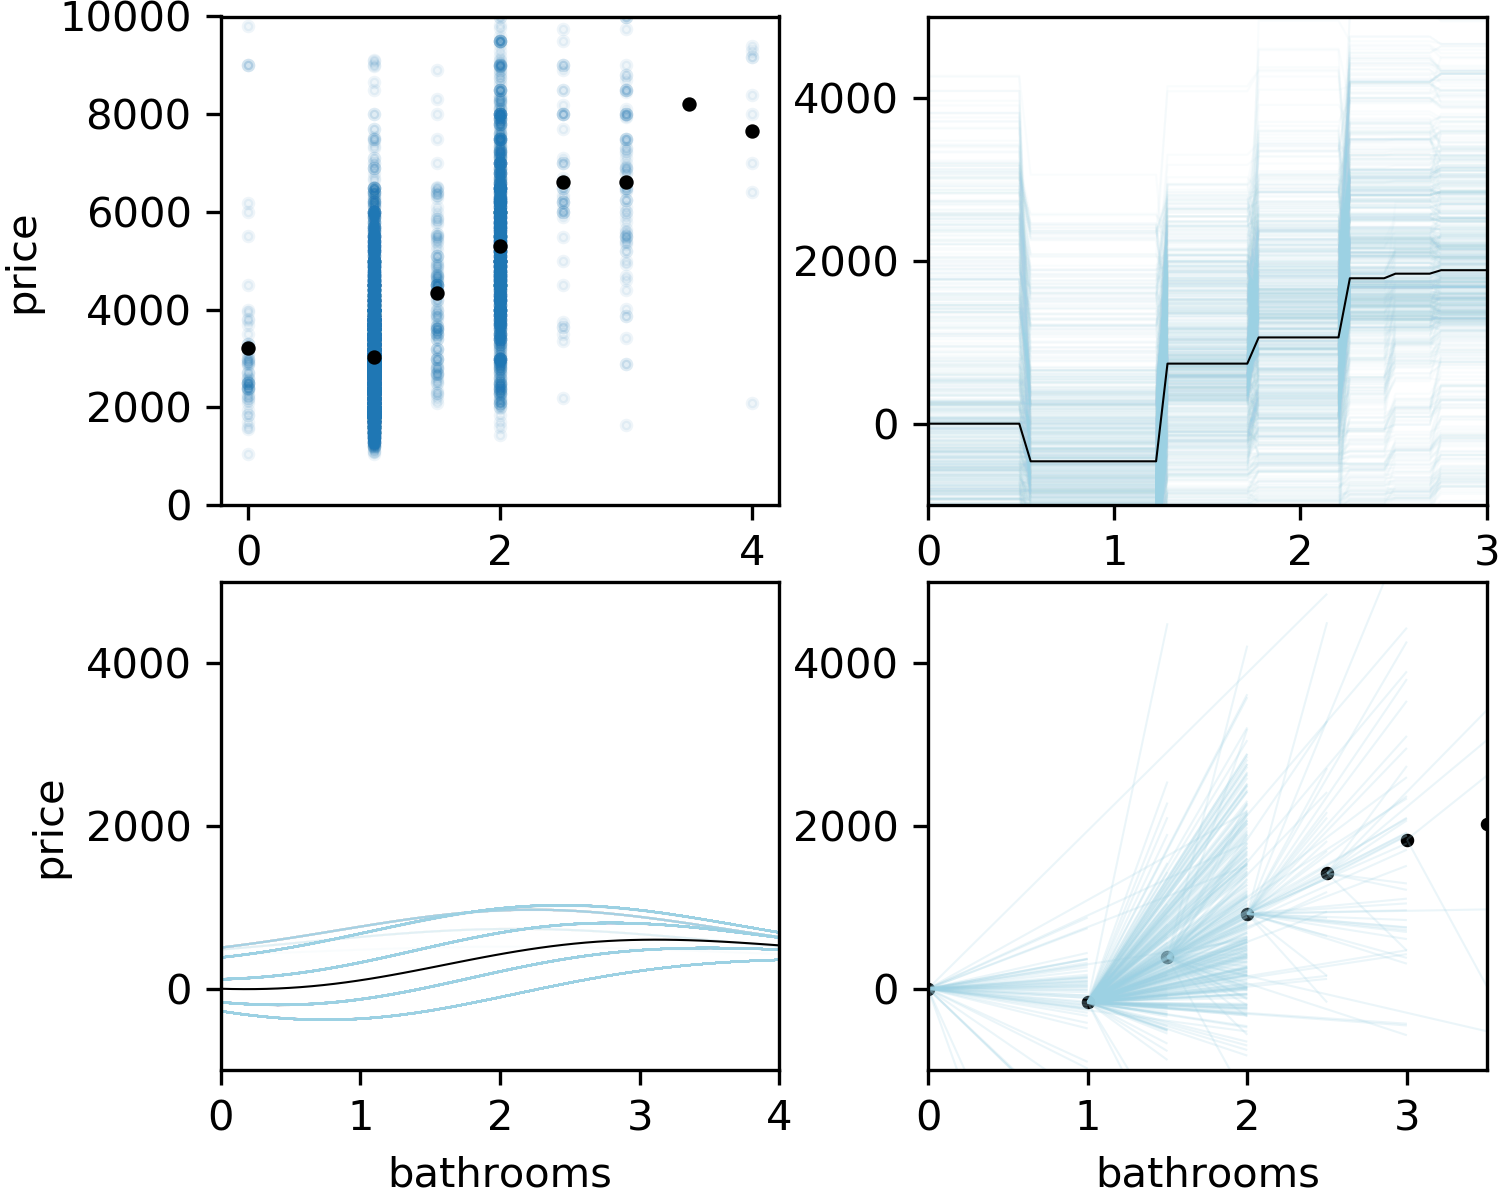
\includegraphics[scale=0.7]{images/bathrooms_vs_price.png}
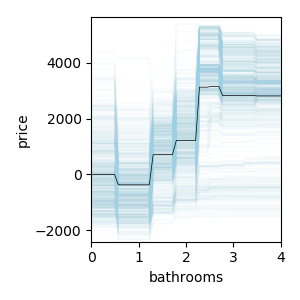
\includegraphics[scale=0.7]{images/bathrooms_vs_price_pdp.png}
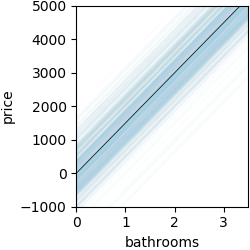
\includegraphics[scale=0.7]{images/bathrooms_vs_price_pdp_lm.png}
\caption{{\bf  Marginal plot and PDP/ICE plot of bathrooms versus rent price; sample size 8000 of 400k...}}
\label{fig:baths_price}
\end{center}
\end{figure}

\cut{The partial dependence plot broadly follows the marginal plot except for the prices of two and three bathroom apartments, where it levels off. This is counterintuitive and exposes an issue with PD and ICE plots.} While PD and ICE plots are {\em model-agnostic}, they are not {\em model-independent} and are subject to the strengths and weaknesses of the model making predictions.  For example, Random Forests(tm) (RF) cannot extrapolate beyond their support range and this data set subset of 8000 observations has very few apartments with 0 or more than two bathrooms.  (Note the lack of blue dots in those ranges of the marginal plot.) PD and ICE plots shift the bathroom feature of all observations from 0 to 3, accepting less trustworthy predictions from the model in extreme ranges.   

Also, getting radically different PD and ICE plots for different underlying models is undesirable because users cannot distinguish between interesting target fluctuations and artifacts of their model choice. Consider \figref{fig:baths_price}(c) that shows the PD/ICE plot for the exact same data set but using a linear model (with Lasso regularization). At the very least, users should compare plots derived from multiple models. Moreover, PD and ICE plots are only as accurate as the underlying model, meaning PD and ICE plots from derived high-bias models should not be trusted.

There are two remaining issues with PD plots associated with the relationship between features. First, as Friedman pointed out, PD plots are most accurate ``{\em when {\em [the model]} is dominated by low order interactions.}''  Feature interactions such as $x_1x_2$ are difficult to tease apart to obtain partial dependencies on just $x_1$ or $x_2$. (Feature $x_j^T = (x_{1j}, .., x_{Nj})$ is a column vector of the  $N \times p$ explanatory matrix ${\bf X}$). ICE plots address this issue by showing separate prediction curves for each observation as the feature of interest is moved through all possible values.  This not only shows the variation hidden by the PD average curve, but it depicts interaction relationships between the feature of interest and other features. \todo{ref later fig}.

The second issue stems from a lack of independence between features.  In a nutshell, not every combination of dependent features is valid. Consider a five bedroom apartment with just one or even zero bathrooms or a four bathroom studio was no bedroom or an observation identified as male but also pregnant.  Because PD and ICE alter observations by shifting the feature of interest through all possible feature values, they run the risk of conjuring up nonsensical observations, and in our experience, features in real data sets are very often dependent to some degree. This problem can be mitigated by computing PD and ICE plots on groups of mutually-dependent or interacting features of interest. \todo{but could involve identifying subsets and computing lots of combinations and we still might want to know about a single contribution.}

To summarize the hazards of PD and ICE plots, {\em (i)} both are strongly affected by the model chosen by the programmer.  {\em (ii)} To obtain accurate plots, PD and ICE rely on the accuracy of the underlying model, which might sacrifice local accuracy to minimize some global loss function.  Both plots display model prediction results rather than the data itself. {\em (iii)} The potentially inaccurate model feeds off of potentially-nonsensical, synthesized observations arising from variable dependencies. What we need is an accurate mechanism that does not rely on, nor make predictions from, a user's model and a mechanism that does not presume independent features.

\section{Our approach}

In a perfect world, a model-independent approach supporting non-independent and interacting features would be straightforward because we would know the actual function, $y = f({\bf x})$ or ${\bf y} = f(\bf X)$, that precisely maps a feature vector ${\bf x}_i$ to target value $y_i$ where ${\bf x}_i = ( x_{i1}, .., x_{ip} )$ is a $1 \times p$ row vector of $\bf X$. The partial derivative of $f({\bf x})$ with respect to a variable (column) of interest, $x_c^T = (x_{1c}, .., x_{Nc})$, describes how a unit change in $x_c$ affects $y$ for all $x_c$ values, treating all other variables as constants. Integrating the partial derivative $\frac{\partial}{\partial x_{c}} f({\bf x})$ would yield a curve showing just $x_{c}$'s contribution to $y$. 

Even though $y = f(\bf x)$ is unavailable, a linear regression model, $y = \hat{f}(\bf x)$, provides the general trend of $y$ versus feature $x_c$ via regression coefficient $\beta_c$. For a unit change in $x_c$, $y$ increases or decreases by $\beta_c$, effectively canceling out or controlling for the other features, $x_{j}$ for $j \neq c$. \cut{(Let $x_{(-c)} = x_j ~\forall~ j \neq c$)}. There are a few problems with using a global linear model, however.  First, a linear model might not be strong enough to capture the relationship between all $({\bf x}_i, y_i)$ observation pairs. Second, coefficient $\beta_c$ is a constant and smooths over any local $y$ fluctuations across the entire range of $x_c$. Third, linear models require dummy variables to represent (and replace) categorical $x_c$ variables, therefore, regression coefficients describe the relationship between the presence or absence of a single category and $y$, rather than $x_c$ and $y$.

Another simple but impractical approach stratifies a data set, grouping observations by all features except the feature of interest, $x_c$.  Let $G$ be a group of observations, identified by a set of row indices, where each observation has identical $x_{j}$ features for $j \neq c$: $\{((x_{i1}, .., x_{ij \neq c}, .., x_{ip}),  y_i)\}_{i \in G}$. For a given $G$, the $\{(x_{ic},  y_i)\}_{i \in G}$ pairs then partially describe how $x_c$ affects $y$, all else being equal.  Fitting a univariate linear regressor (without regularization) to group $G$ yields an approximation, $\beta_G$, of the slope of $y$ localized to the specific region of $x_c$ in group $G$: $R_G = [min(x_{ic}), max(x_{ic})]_{i \in G}$.   Because the $x_c$ regions from multiple groups could overlap, slope $\beta_R$ in any given $x_c$ region, $R$, would be the average of all slope estimates covering that region: $\beta_R = \frac{1}{|G \in R|}\Sigma_{G \in R}\beta_G$. Together, the collection of regions and slopes, $\{(R, \beta_R)\}_{R \in x_c}$, would cover the full $x_c$ range and represent a good localized approximation of the partial derivative of the unknown $f(\bf x)$ with respect to $x_c$.

Alas, this stratification approach works for two or three variables but breaks down for more variables because it is impractical to find groups of observations that are equal across so many variables.  Nonetheless, stratification is simple, well understood, and clearly isolates the effect of $x_c$ on $y$ from the other features for this application, even in the presence of non-independent and interacting features.  The only obstacle is a general and practical mechanism for stratifying observations with many variables, which leads us to the primary contribution of this paper.

The key idea is to relax stratification so that it organizes observations into groups of similar rather than equal observations.  Our approach, called \spd, uses a random forest to stratify observations into  groups of similar observations and then collects piecewise linear approximations to the partial derivatives of the unknown $f(\bf x)$ for the groups. Each leaf, $L$, in each tree of the forest represents a group with similar $x_{(-c)}$ values and yields a $\beta_L$ from a linear model trained on $(Lx, Ly)$, the $x_c$ and $\bf y$ observations associated with $L$.  The partial derivative between any two (unique and sorted) adjacent $x_c$ data points is estimated by averaging the $\beta_L$ coefficients that overlap that range, yielding $n-1$ partial derivatives for $n$ unique $x_c$ values.  Numerically integrating the partial derivatives across $x_c$ space gives a curve representing the contribution of $x_c$ to $y$. This process is depicted in \figref{fig:leaves}. There are five leaves in \figref{fig:leaves}, potentially from multiple trees in a forest, with regression lines fit through leaf observations, $(Lx, Ly)$. The $x_c$ values in $L_5$ are identical so its infinite slope is ignored.

\begin{figure}[htbp]
\begin{center}
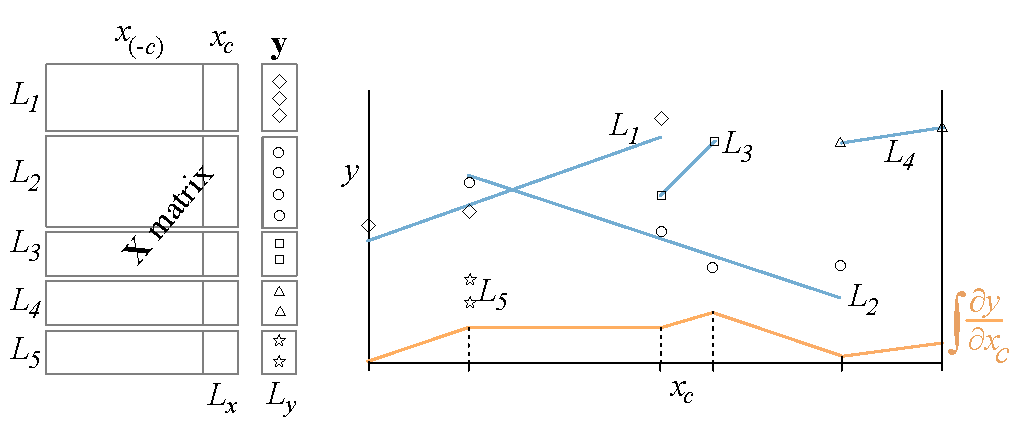
\includegraphics[scale=0.7]{images/leaves.pdf}
\caption{{\bf  Leaves $L_i$...}}
\label{fig:leaves}
\end{center}
\end{figure}

\spd{} trains a random forest in the usual way but on $({\bf X}_{(-c)}, {\bf y})$ rather than $({\bf X}, {\bf y})$, where ${\bf X}_{(-c)}$ = $\{(x_1, .., x_{i \neq c}, .., x_p)\}_{i=1}^N$ is the explanatory matrix {\em without} column vector $x_c$.  Observations $({\bf x}_{i}, y_i)$ that end up in a tree leaf are more likely than not to be similar, but similar only in columns $x_{(-c)}$ since the forest trained on ${\bf X}_{(-c)}$. (\todo{cite breiman similarity mechanism}.)   Training must ensure individual decision trees in the forest have at least two samples per leaf in order to fit localized linear models. With too few observations in leaf $L$, $\beta_L$ is a poor estimate; with too many, $\beta_L$ is overly-sensitive to contributions from non-$x_c$ features. \spd{} degenerates to a simple marginal plot if training yields a single tree with a single node containing all of $\bf X_{(-c)}$.  

\begin{figure}[htbp]
\begin{center}
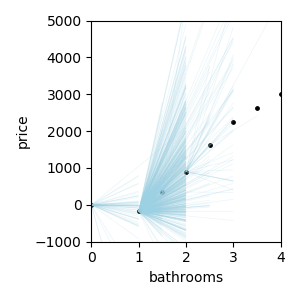
\includegraphics[scale=0.7]{images/bathrooms_vs_price_stratpd.png}
\caption{{\bf  \spd{} partial dependence plot of bathrooms versus rent price}}
\label{fig:baths_price_stratpd}
\end{center}
\end{figure}

\figref{fig:baths_price_stratpd} shows the \spd{} plot derived from the same apartment rent data set used by the PD/ICE plots in \figref{fig:baths_price}. Each blue line represents the regression line through the observations in a single leaf of observations with similar $x_{(-c)}$ features. Dropping the $y$-intercept from the regression line effectively drops the contributions of $x_{(-c)}$ features to $Ly$.  The emanating and terminating $x$ positions of $L$'s line are the minimum and maximum $x_c$ in $L$, $R_L$. The height of $L$'s line is $\beta_G \Delta{}R_L$, the slope times the width of region $R_L$. The black dots represent the integration of the $\beta_R$ values at $x_c$.

interesting: starts at 0 at min $x_c$, variation in dx at each $x_c$, density of data, only shows at $x_c$

Algorithm \ref{alg:StratPD}...

\setlength{\algomargin}{5pt}
\begin{algorithm}[H]
\label{alg:StratPD}
\LinesNumbered
\SetAlgorithmName{Algorithm}{List of Algorithms}
\SetAlgoSkip{}
\SetInd{.5em}{.5em}
\TitleOfAlgo{{\em StratPD}($X$, $\bf y$, $c$) {\bf returns} collection of $\beta$ coefficients, $\hat{y}$}
Train random forest regressor {\it rf} on (${\bf X}_{(-c)}$, $\bf y$)\\
\ForEach{leaf $L \in {\it rf}$}{
	$(Lx, Ly)$ = $\{(x_{ic},  y_i)\}_{i \in L}$\\
	$R_L$ = $[min(Lx), max(Lx)]$\\
	\lIf{left$(R_L)$ = right$(R_r)$}{{\bf continue}}\\
	Fit linear model to $(Lx, Ly)$ giving $\beta_L$\\
}
$uniqx$ = sorted(unique($x_c$))\\
\For{$i=1$ {\bf to} $|uniqx|-1$}{
	$R$ = $(uniqx_i, uniqx_{i+1})$\\
	\ForEach{leaf $L \in {\it rf}$}{
		$\beta_{R} = \frac{1}{|R_L \in R|}\Sigma_{R_L \in R}\beta_L$\\
	}
}
$\hat{y}$ = numerically integrate $\beta_R$'s at $uniqx$ leaving first integral value as y=0\\
\Return{collection of all $\beta_R$ and $\hat{y}$}
\end{algorithm}

{\em this is transition to categorical...} Besides enabling stratification of $\bf X$, random forests do not require one-hot encoding of categorical variables, treating categories as unique integers. Algorithm \ref{alg:CatStratPD}...

\setlength{\algomargin}{5pt}
\begin{algorithm}[H]
\label{alg:CatStratPD}
\LinesNumbered
\SetAlgorithmName{Algorithm}{List of Algorithms}
\SetAlgoSkip{}
\SetInd{.5em}{.5em}
\TitleOfAlgo{{\em CatStratPD}($X$, $\bf y$, $c$) {\bf returns} dictionary mapping category to $y$}
Train random forest regressor {\it rf} on (${\bf X}_{(-c)}$, $\bf y$)\\
Let $D$ be dictionary mapping category to $y$ value\\
\ForEach{leaf $L \in {\it rf}$}{
	$(Lx, Ly)$ = $\{(x_{ic},  y_i)\}_{i \in L}$\\
	\ForEach{$cat \in Lx$}{
		$cat_y$ = $Ly[Lx=cat]$\\
		\lIf{$|cat_y| < 2$}{{\bf continue}}\\
		$cat_{avg}$ = $\frac{1}{|cat_y|} \Sigma cat_y$\\
		$cat_{avg}$ = $cat_{avg} - min(Ly)$~~~~~~(Strip y contribution from $x_{(-c)}$)\\
		$D_{cat}$ = $D_{cat} + cat_{avg}$\\
	}
}
Let $n_{cat}$ be number of $cat_{avg}$ added to $D_{cat}$\\
$D_{cat}$ = $D_{cat} / n_{cat}$~~~~(Take average of leaf averages for $cat$)\\
\Return{$D_{cat}$}
\end{algorithm}


Region endpoints are limited to $x_{ic}$ points from the training data $\bf X$.  There is no interpolation between points, though we use the slope to summarize the relationship of $y$ to $x_c$ in $R$.

no conjuring of synthetic observations

less sensitive to nonindependent variables.
 
few data points in leaves. parameterized slope provides better estimate

randomization means of controlling for confounding variables

combine derivative in the same plot

since we care most about how y changes per changes in $x_i$, absolute plots are less useful than relative plots; compare with centered ICE, which I also don't like.

\section{Experimental Results}

\begin{figure}[htbp]
\begin{center}
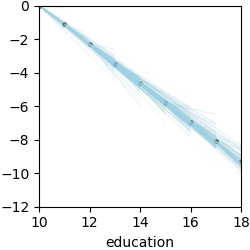
\includegraphics[scale=0.7]{images/education_vs_weight_stratpd.png}
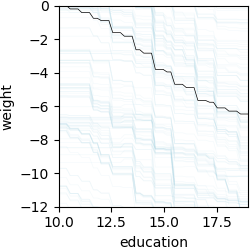
\includegraphics[scale=0.7]{images/education_vs_weight_pdp.png}
\caption{{\bf  Edu vs weight}}
\label{fig:education_vs_weight}
\end{center}
\end{figure}

\begin{figure}[htbp]
\begin{center}
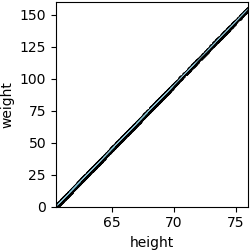
\includegraphics[scale=0.7]{images/height_vs_weight_stratpd.png}
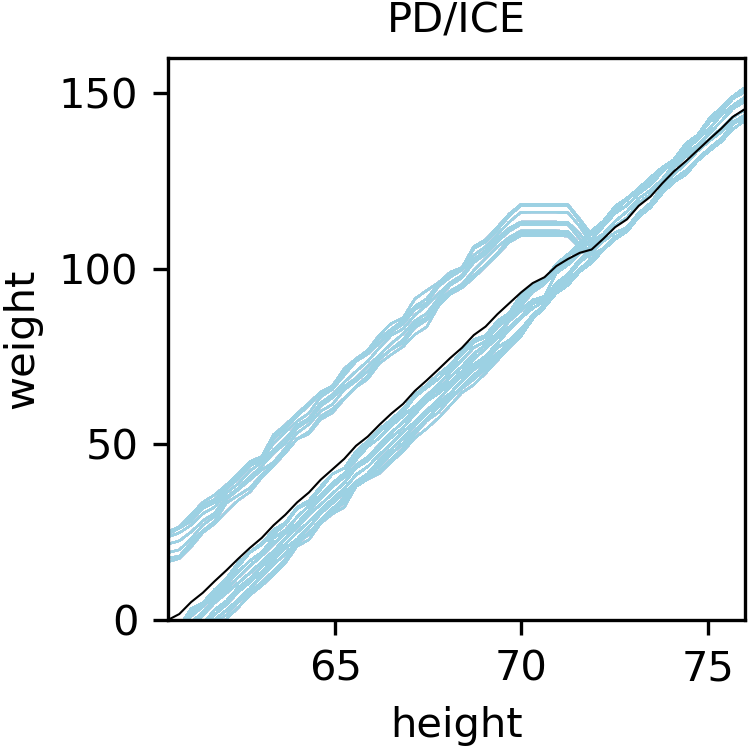
\includegraphics[scale=0.7]{images/height_vs_weight_pdp.png}
\caption{{\bf  Height vs weight}}
\label{fig:height_vs_weight}
\end{center}
\end{figure}

\begin{figure}[htbp]
\begin{center}
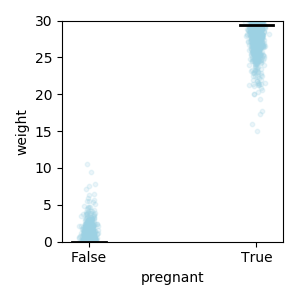
\includegraphics[scale=0.7]{images/pregnant_vs_weight_stratpd.png}
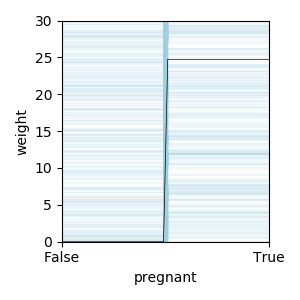
\includegraphics[scale=0.7]{images/pregnant_vs_weight_pdp.png}
\caption{{\bf  pregnant vs weight}}
\label{fig:pregnant_vs_weight}
\end{center}
\end{figure}

\begin{figure}[htbp]
\begin{center}
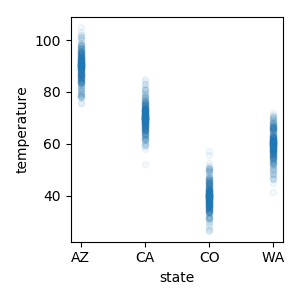
\includegraphics[scale=0.7]{images/state_vs_temp.png}
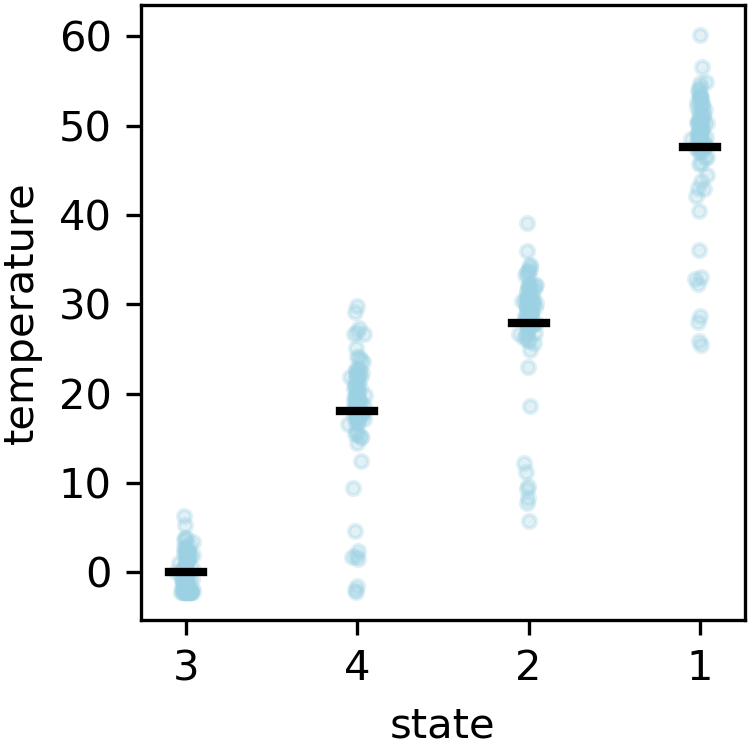
\includegraphics[scale=0.7]{images/state_vs_temp_stratpd.png}
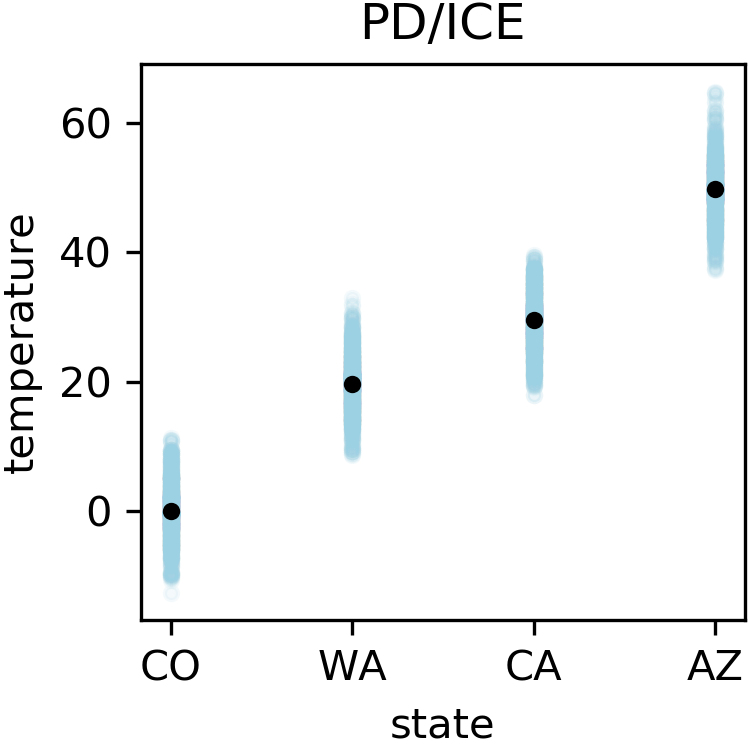
\includegraphics[scale=0.7]{images/state_vs_temp_pdp.png}
\caption{{\bf  state  vs temp}}
\label{fig:state_vs_temp}
\end{center}
\end{figure}

\begin{figure}[htbp]
\begin{center}
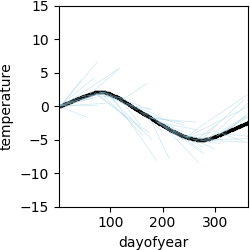
\includegraphics[scale=0.7]{images/dayofyear_vs_temp_stratpd.png}
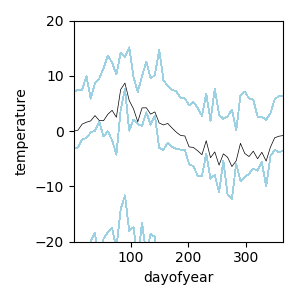
\includegraphics[scale=0.7]{images/dayofyear_vs_temp_pdp.png}
\caption{{\bf  dayofyear  vs temp}}
\label{fig:dayofyear_vs_temp}
\end{center}
\end{figure}

\begin{figure}[htbp]
\begin{center}
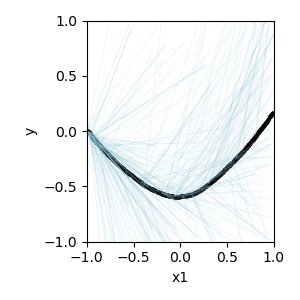
\includegraphics[scale=0.7]{images/add_x1_y_stratpd.png}
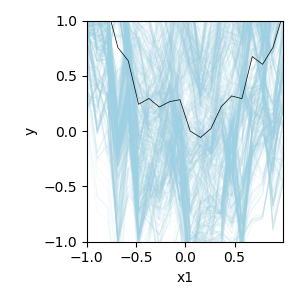
\includegraphics[scale=0.7]{images/add_x1_y_pdp.png}
\\
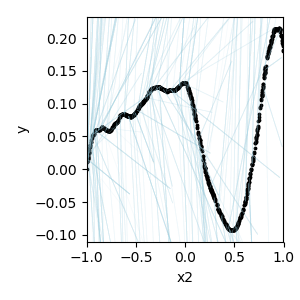
\includegraphics[scale=0.7]{images/add_x2_y_stratpd.png}
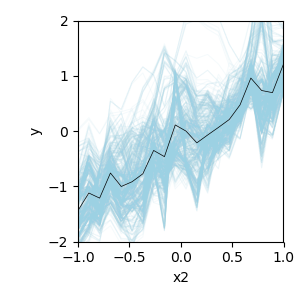
\includegraphics[scale=0.7]{images/add_x2_y_pdp.png}
\caption{{\bf  additive from ICE x1, x2 vs y; $y = x_1^2 + x_2 + \epsilon$, $x_1, x_2, x_3$ are U(-1,1) Sample size 1000}}
\label{fig:add_x1_y_stratpd}
\end{center}
\end{figure}

\begin{figure}[htbp]
\begin{center}
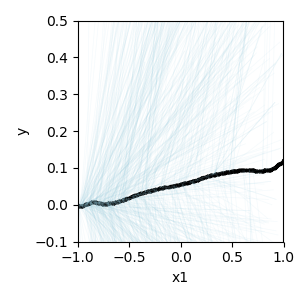
\includegraphics[scale=0.7]{images/bigx_x1_y_stratpd.png}
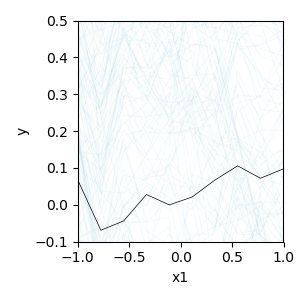
\includegraphics[scale=0.7]{images/bigx_x1_y_pdp.png}
\\
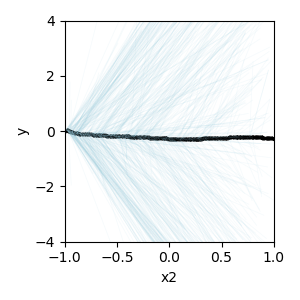
\includegraphics[scale=0.7]{images/bigx_x2_y_stratpd.png}
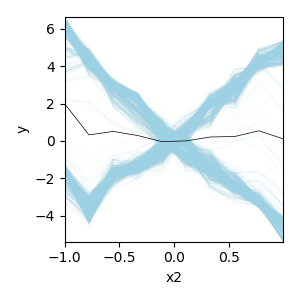
\includegraphics[scale=0.7]{images/bigx_x2_y_pdp.png}
\\
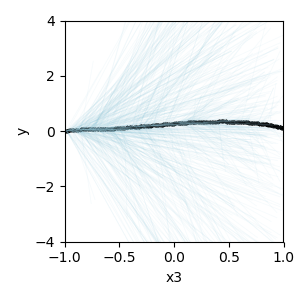
\includegraphics[scale=0.7]{images/bigx_x3_y_stratpd.png}
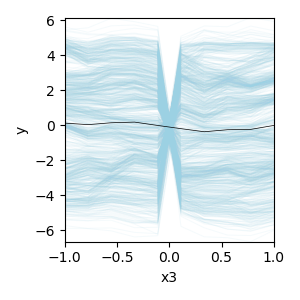
\includegraphics[scale=0.7]{images/bigx_x3_y_pdp.png}
\caption{{\bf  big X from ICE $y = 0.2x_1 - 5x_2 + 10x_2\mathbf{1}_{x_3 \geq 0} + \epsilon$, $x_1, x_2, x_3$ are U(-1,1), Sample size 1000}}
\label{fig:add_x1_y_stratpd}
\end{center}
\end{figure}

\section{Related Work}

There are a few basic approaches to identifying the partial effect of a single variable on the target or response variable:

\begin{itemize}
\item Stratification
\item Beta coefficients from linear model without regularization
\item Marginal plots
\item PDP/ICE
\item Accumulated Local Effects (https://arxiv.org/abs/1612.08468) (ALE) plots
\end{itemize}

PDP math shows that features added or multiplied times the remaining F approximation completely describe the partial dependence; I assume that means that interactions are not a problem.

do we need to talk about LIME?

there are other ways to stratify X, such as quartiles or binning of some kind but we have to choose the bins or the similarity measure.

propensity stuff James mentioned

talk about how we do not presume independence of features
 
This python package seems to do PDP, LIME etc... https://github.com/oracle/Skater

\section{Future work}

This work describes regressors only, ignoring partial dependence for classifiers.  Research reveals no papers or implementation for classifiers. Friedman, however, briefly describes a partial dependence mechanism for classification whereby $k$-class logistic regression (one-versus-rest) equations indicate the probability of seeing class $k$ at $\bf{x}$.  This suffers from the same interaction-based bias as the regressor model.

Actually, the R version of personal dependence may actually do this. See https://christophm.github.io/interpretable-ml-book/pdp.html where he describes PDP for cancer prediction and gets probabilities out.

\section{Conclusion}
\label{sec:conc}

\bibliographystyle{apalike}

\bibliography{stratpd}
\end{document}